\chapter{Controle Bancário: Versão 2}\label{autenticacao}

Neste  capítulo,   dando  continuidade   ao  desenvolvimento  em   Grails,  será
apresentado o  processo de desenvolvimento  da segunda versão da  aplicação {\bf
  ControleBancario}. Nessa versão são incorporadas as seguintes funcionalidades:

\begin{itemize}

\vspace{0.5cm}

\item Controle de acesso: autenticação e autorização de usuários;

\vspace{0.5cm}

\item  Internacionalização. Ou  seja,  personalizar o  conteúdo apresentado  nas
  visões (*.gsp) com base no {\it Locale} (idioma e região) dos usuários;

\vspace{0.5cm}

\item  Personalização dos  {\it  templates} utilizados  pelo  mecanismo de  {\it
  scaffolding} na geração dos controladores e visões;

\vspace{0.5cm}

\item Definição  de máscaras de entrada para  os atributos CEP, CNPJ,  e CPF das
  classes de domínio; e 

\vspace{0.5cm}

\item  Implementação de  uma biblioteca  de marca\footnote{Em  inglês:  {\it tag
    library.}} que apresenta informações relacionadas ao usuário logado. 

\end{itemize}

\section{Configuração da aplicação} 

\vspace{0.5cm}

\noindent{\bf (a) Instalação de  plugins.}  Na implementação das funcionalidades
da aplicação {\bf ControleBancario}, discutidas nesse capítulo, será utilizado o
plugin Grails {\bf  spring-security} que auxilia a autenticação  dos usuários da
aplicação.\index{Plugins!spring-security} 

Conforme discutido  anteriormente, para instalar o  plugin {\bf spring-security}
adicione   uma    linha,   descrevendo   a   dependência,    no   arquivo   {\bf
  BuildConfig.groovy}     conforme     apresentado     na    linha     51     do
Código~\ref{codBuildConfig2}.   Porém,  desde  que  o código  fonte  desse  {\it
  plugin}  encontra-se  no repositório  da  {\it  Spring},  é necessário  também
configurar  o endereço  desse repositório  conforme apresentado  na linha  23 do
Código~\ref{codBuildConfig2}.  

\vspace{0.5cm}

\noindent{\bf (b)  Instalação de bibliotecas Javascript.}   Na implementação das
funcionalidades discutidas nesse capítulo, serão utilizadas as bibliotecas: {\bf
  jquery-1.8.3.min.js}   e  {\bf  jquery.maskedinput.min.js}   que  encontram-se
disponíveis                 no                 seguinte                endereço:
{\footnotesize\url{http://www.dc.ufscar.br/~delano/ControleBancario/}}.     Dessa
forma, é necessário  fazer o {\it download} desses dois  arquivos e copiá-los no
diretório {\bf web-app/js}.  O  diretório {\bf web-app} encontra-se no diretório
raiz da aplicação {\bf ControleBancario}. 

\vspace{0.5cm}

\noindent{\bf  (c)  Atualização  das   dependências.}   Por  fim,  é  necessário
atualizar as  dependências ({\it plugins}) da  aplicação {\bf ControleBancario}.
Para  tal, no  IDE GGTS:  Selecione  {\bf Grails  Tools} $\Longrightarrow$  {\bf
  Grails  Command Wizard}.   Digite {\bf  refresh-dependencies} como  o  nome do
comando  a ser  executado e  clique  em {\bf  Next}.  Esse  comando atualiza  as
dependências    e     instala    os    {\it     plugins},    caso    necessário.
\index{Comandos!grails refresh-dependencies} 

\begin{lstlisting}[numbers=left, caption={\bf BuildConfig.groovy}, frame = trBL,
    float=htbp, label=codBuildConfig2]
grails.project.dependency.resolution = {
    // inherit Grails' default dependencies
    inherits("global") {
        // specify dependency exclusions here; for example, uncomment this to disable ehcache:
        // excludes 'ehcache'
    }
    log "error" // log level of Ivy resolver, either 'error', 'warn', 'info', 'debug' or 'verbose'
    checksums true // Whether to verify checksums on resolve
    legacyResolve false 

    repositories {
        inherits true // Whether to inherit repository definitions from plugins

        grailsPlugins()
        grailsHome()
        mavenLocal()
        grailsCentral()
        mavenCentral()
        // uncomment these (or add new ones) to enable remote dependency resolution from public Maven repositories
        //mavenRepo "http://repository.codehaus.org"
        //mavenRepo "http://download.java.net/maven/2/"
        //mavenRepo "http://repository.jboss.com/maven2/"
        mavenRepo "http://repo.spring.io/milestone/"
    }

    dependencies {
        // specify dependencies here under either 'build', 'compile', 'runtime', 'test' or 'provided' scopes e.g.
        // runtime 'mysql:mysql-connector-java:5.1.27'
        runtime 'org.postgresql:postgresql:9.3-1100-jdbc41'
    }

    plugins {
        // plugins for the build system only
        build ":tomcat:7.0.50"

        // plugins for the compile step
        compile ":scaffolding:2.0.1"
        compile ':cache:1.1.1'

        // plugins needed at runtime but not for compilation
        runtime ":hibernate:3.6.10.7" // or ":hibernate4:4.1.11.6"
        runtime ":database-migration:1.3.8"
        runtime ":jquery:1.10.2.2"
        runtime ":resources:1.2.1"
        // Uncomment these (or add new ones) to enable additional resources capabilities
        //runtime ":zipped-resources:1.0.1"
        //runtime ":cached-resources:1.1"
        //runtime ":yui-minify-resources:0.1.5"
        
        compile ":br-validation:0.3"
        compile ":spring-security-core:2.0-RC2"
    }
}
\end{lstlisting}

\newpage

\section{Controle de Acesso}

\vspace{0.3cm}

Conforme dito,  a segunda versão  da aplicação {\bf ControleBancario}  utiliza o
{\it                                 plugin}                                {\bf
  spring-security-core}\footnote{\url{http://grails.org/plugin/spring-security-core}}
que          simplifica         a          integração          do         Spring
Security\footnote{\url{http://static.springsource.org/spring-security/site/index.html}}
em aplicações Grails. \index{Plugins!spring-security} 

\vspace{0.3cm}

Esse {\it plugin}  define uma série de comandos. Entre  esses podemos destacar o
comando {\bf s2-quickstart}  que cria tanto as classes  de domínio básicas tanto
os  controladores (e  suas  respectivas  visões) necessários  para  lidar com  a
autenticação de usuários. 

\vspace{0.3cm}

Portanto, o  primeiro passo  na implementação da  funcionalidade de  controle de
acesso é a execução desse comando.  Para tal, no IDE GGTS: Selecione {\bf Grails
  Tools}   $\Longrightarrow$   {\bf  Grails   Command   Wizard}.   Digite   {\bf
  s2-quickstart} como o nome do comando  a ser executado e clique em {\bf Next}.
Digite  {\bf br.ufscar.dc.dsw  Usuario Papel}  como os  parâmetros do  comando e
clique    em     {\bf    Next}.      Esse    comando    cria     os    seguintes
artefatos:\index{Comandos!grails s2-quickstart} 

\vspace{0.5cm}

\begin{itemize}

\item  {\bf br.ufscar.dc.dsw.Usuario}  -- classe  de domínio  que  representa os
  usuários autenticados. 

\vspace{0.3cm}

\item {\bf br.ufscar.dc.dsw.Papel} -- classe de domínio que representa os papéis
  que  os  usuários  podem  desempenhar.  Cada papel  possui  permissões  a  ele
  associadas.  

\vspace{0.5cm}

\item {\bf br.ufscar.dc.dsw.UsuarioPapel} --  classe de domínio que representa o
  relacionamento  muitos-para-muitos  entre  usuários  e papéis.   Ou  seja,  um
  usuário pode  desempenhar vários papeis e  um papel pode  ser desempenhado por
  vários usuários. 

\vspace{0.5cm}

\item {\bf LoginController} e {\bf LogoutController} (e suas respectivas visões)
  que  são  responsáveis  pelas operações  de  {\it  login}  e {\it  logout}  da
  aplicação.

\end{itemize}

\vspace{0.5cm}

A seguir, adicione  o seguinte trecho na classe de domínio  {\bf Usuario} -- pai
da  hierarquia de  usuários  da  aplicação {\bf  ControleBancario}.  Ou seja,  a
estratégia  de mapeamento  {\it table-per-hierarchy}  (Seção~\ref{secGORM}) será
desabilitada   e,  para   essa  hierarquia   de  classes,   a   estratégia  {\it
  table-per-class} será  utilizada.  Assim,  é criada uma  tabela para  a classe
{\bf Usuario} assim como para cada classe filha discutida nas próximas seções.

\vspace{0.5cm}

\begin{cBox}
\begin{small}
\begin{verbatim}
static mapping = {
    password column: '`password`'
    tablePerHierarchy false
}
\end{verbatim}
\end{small}
\end{cBox}

\vspace{0.5cm}

Por fim,  adicione o seguinte  trecho no arquivo {\bf  conf/Config.groovy}. Esse
comando  habilita  que  os  comandos  \texttt{HTTP POST}  e  \texttt{GET}  sejam
utilizados para  invocar o controlador {\bf LogoutController}  que é responsável
pela operação de {\it logout} da  aplicação. Por {\it default}, apenas o comando
\texttt{POST}   pode   ser   utilizado   para   invocar   o   controlador   {\bf
  LogoutController}. 

\vspace{0.5cm}

\begin{cBox}
\begin{small}
\begin{verbatim}
grails.plugin.springsecurity.logout.postOnly = false
\end{verbatim}
\end{small}
\end{cBox}

\newpage

\subsection{Classes de Domínio: Cliente, ClienteFisico, ClienteJuridico e Gerente}

Os    clientes   e   os    gerentes   serão    usuários   da    aplicação   {\bf
  ControleBancario}.  Ou  seja, as  classes  de  domínio  {\bf Cliente}  e  {\bf
  Gerente}   são  subclasses  da   classe  {\bf   Usuario}  definida   na  seção
anterior. Desde que  as classes {\bf ClienteFisico} e  {\bf ClienteJuridico} são
subclasses de {\bf Cliente}, estas também serão subclasses de {\bf Usuario}.

A classe {\bf Usuario} define dois atributos {\bf username} e {\bf password} que
são  responsáveis pelo  armazenamento do  {\it login}  e senha  dos  usuários da
aplicação.   Código~\ref{codUsuario}  mostra   as  alterações  na  implementação
das  classes {\bf Cliente},  {\bf ClienteFisico},  {\bf ClienteJuridico}  e {\bf
  Gerente}.   Pode-se  observar  que   na  implementação  dessas  classes  foram
incluídas  restrições   relacionadas  aos   atributos  {\bf  username}   e  {\bf
  password} definidos pela classe pai {\bf Usuario}. 

\begin{lstlisting}[caption=Usuários:   Clientes  e   Gerentes,  frame   =  trBL,
    float=htbp, label=codUsuario] 
abstract class Cliente extends Usuario {  
 
   static constraints = {
        username (blank: false, unique: true)
        password (password: true, blank: false)
        // demais restri^çõ^es
    }

    // atributos e m^é^todos da classe
}

class ClienteFisico extends Cliente {
    
    static constraints = {
        username (blank: false, unique: true)
        password (password: true, blank: false)
        // demais restri^çõ^es
    }
    
    // atributos e m^é^todos da classe
}

class ClienteJuridico extends Cliente {
    
    static constraints = {
        username (blank: false, unique: true)
        password (password: true, blank: false)
        // demais restri^çõ^es
    }
    
   // atributos e m^é^todos da classe
}

class Gerente extends Usuario {

    static constraints = {
        username (blank: false, unique: true)
        password (password: true, blank: false)
        // demais restri^çõ^es
    }
   
    // atributos e m^é^todos da classe
}
\end{lstlisting}

\section{Internacionalização}\label{I18n}
\index{Internacionalização~-~I18n}

Grails  apoia a internacionalização  (i18n). Ou  seja, com  o Grails  é possível
personalizar o conteúdo  que aparece em qualquer visão (*.gsp)  com base no {\it
  Locale} dos usuários. 

Para  tirar proveito do  suporte a  internacionalização em  Grails, a  equipe de
desenvolvimento tem que criar {\it message  bundles} -- uma para cada idioma que
a  equipe  deseja  internacionalizar.  {\it  Message bundles}  em  Grails  estão
localizados  dentro  do   diretório  {\bf  i18n}  e  são   simples  arquivos  de
propriedades    Java/Groovy.     Por   padrão,    Grails    procura   em    {\it
  messages.properties} para mensagens, a menos que o usuário tenha especificado 
um {\it Locale} em específico. A equipe de desenvolvimento pode criar novas {\it
  message  bundles}  simplesmente criando  novos  arquivos  de propriedades  que
terminam   com  a   localidade   que  está   interessada.   Por  exemplo,   {\it
  messages\_pt\_BR.properties}      para     o      Português      do     Brasil
(Figura~\ref{I18nFig}).

\begin{small}
\begin{cBox}
Um objeto {\it Locale} representa  uma região geográfica específica, político ou
cultural. Uma  operação que requer uma  localidade para executar a  sua tarefa é
denominada de sensível e usa o objeto {\it Locale} para prover a informação mais
apropriada aos  usuários. Por exemplo,  exibir o preço  de uma mercadoria  é uma
operação sensível a  localidade -- o número deve ser formatado  de acordo com os
costumes e convenções do país de origem do usuário, região ou cultura.

O objeto {\it Locale} é composto por:  (i) um código do idioma ou (ii) um código
do idioma e  um código de país. Por  exemplo, {\bf en} é o código  para o idioma
Inglês (não importando o país ou região geográfica) enquanto {\bf pt\_BR} e {\bf
  pt\_PT} são dois {\it Locales} que compartilham o mesmo idioma: o primeiro é o
código para o Português do Brasil e  o segundo é o código para o Português usado
em Portugal (Figura~\ref{I18nFig}).
\end{cBox}
\end{small}

\begin{figure}[\textit{}htb]
\centering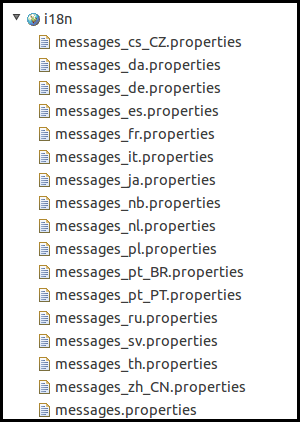
\includegraphics[width=4.5cm]{messages}
\caption{I18n (arquivos de propriedades).}
\label{I18nFig}
\end{figure}

As visões  geradas no  {\it scaffolding} de  nossa aplicação  estão parcialmente
internacionalizados. Ou seja,  pode-se observar que essas visões  incluem a {\it
  tag} {\bf  <g:message code>}, onde code é  uma referência a algum  termo a ser
internacionalizado.   O  nó  {\bf  i18n}  contém  um  conjunto  de  arquivos  de
propriedades   (termos   a  serem   traduzidos   para   diferentes  línguas)   –
Figura~\ref{I18nFig}.   É importante  salientar que  esses arquivos  são gerados
automaticamente  durante a execução  dos comandos  do Grails  ({\bf create-app},
{\bf create-controller}, {\bf generate-all}, etc).  

\begin{small}
\begin{cBox}
As   visões   são   os   locais   mais   comuns  para   o   uso   de   mensagens
internacionalizadas.  Para acessar  as  mensagens personalizadas  nas visões,  a
equipe de desenvolvimento basta utilizar a seguinte {\it tag} nas visões (*.gsp)
desenvolvidas: 

\vspace{0.2cm}

\verb#<g:message code="welcome.greeting" />#

\vspace{0.2cm}

\noindent Se  a equipe tiver  incluido uma chave no  arquivo messages.properties
(com  sufixo do {\it  Locale} apropriado),  tal como  ilustrada a  seguir, então
Grails apresenta a mensagem personalizada:

\vspace{0.2cm}

\verb#welcome.greeting = Good Morning. My name is Bob.#

\vspace{0.2cm}

\noindent Note  que em  algumas ocasiões é  necessário passar argumentos  para a
mensagem. Isso também é possível com a mesma {\it tag}:

\vspace{0.2cm}

\verb#<g:message code="welcome.greeting" args="${ ['Night','Bill'] }" />#

\vspace{0.2cm}

\noindent No entanto,  é necessário utilizar os parâmetros  de posicionamento na
mensagem.

\vspace{0.2cm}

\verb#welcome.greeting = Good {0}. My name is {1}.#
\end{cBox}
\end{small}

\vspace{0.2cm}
\noindent Note que o esforço  da equipe Web para internacionalizar sua aplicação
consiste em determinar  os termos a serem traduzidos, que  serão inseridos em um
arquivo  de  propriedades, e  depois  realizar  a  tradução para  as  diferentes
línguas.  As traduções serão armazenadas  em arquivos cujos nomes terminam com o
{\it Locale} (língua e região) desejado.

Figura~\ref{Agenda18nFig} apresenta algumas mensagens relacionadas às classes de
domínio  {\bf  Agencia}   que  foram  traduzidas  e  copiadas   para  o  arquivo
messages\_pt\_BR.properties   ({\it  Message   Bundle}  para   o   Português  do
Brasil).  Pode-se observar  que esse  arquivo contém  traduções para  o  nome da
classe assim como  para o nome de  cada um de seus atributos.  Além disso, foram
adicionadas  algumas mensagens  relacionadas à  página  de {\it  login} que  foi
gerada automaticamente pela execução do comando {\bf s2-quickstart}. 

\begin{figure}[htbp]
\begin{mdframed}
\begin{footnotesize}
\begin{verbatim}
# Agencia - mensagens
agencia.label = Agência
agencia.numero.label = Número
agencia.nome.label = Nome
agencia.endereco.label = Endereço
agencia.banco.label = Banco
agencia.gerentes.label = Gerentes

# Página de Login - mensagens
springSecurity.login.header = Login
springSecurity.login.remember.me.label = Lembre-me
springSecurity.login.button = Login
springSecurity.login.username.label = Login
springSecurity.login.password.label = Password
\end{verbatim}
\end{footnotesize}
\end{mdframed}
\caption{Messagens I18n para a classe de Domínio Usuario}
\label{Agenda18nFig}
\end{figure}

\begin{remark}
Um  bom exercício  consiste em  internacionalizar as  mensagens  relacionadas às
demais classes de domínio da aplicação {\bf ControleBancario}.  
\end{remark}

\section{Personalização dos templates utilizados no scaffolding}

Nessa seção  será apresentado o  processo de personalização dos  {\it templates}
utilizados pelo  mecanismo de {\it  scaffolding} na geração dos  controladores e
visões. No  contexto da aplicação {\bf  ControleBancario}, essas personalizações
tem  como   objetivo  gerar  os  controladores  e   visões  com  funcionalidades
relacionadas ao controle de acesso já incorporadas. Além disso, a personalização
é  realizada de  tal forma  que  as visões  {\bf create.gsp}  e {\bf  edit.gsp},
geradas pelo  {\it scaffolding},  já incorporam as  máscaras de entrada  para os
atributos CEP, CNPJ e CPF.

Portanto, o primeiro passo no  processo de personalização dos templates consiste
na execução  do comando  {\bf install-templates}.  No  IDE GGTS:  Selecione {\bf
  Grails  Tools} $\Longrightarrow$  {\bf  Grails Command  Wizard}.  Digite  {\bf
  install-templates} como  o nome do  comando a ser  executado e clique  em {\bf
  Next}.  Esse comando copia os {\it templates} usadas nas atividades de geração
de  código  para  o  diretório  {\bf  src/templates}.   Esse  diretório  inclui:
\index{Comandos!grails install-templates} 

\begin{itemize}

\vspace{0.2cm}

\item O  diretório {\bf  artifacts} contém os  {\it templates}  utilizados pelos
  comandos      \texttt{create-*}      ({\bf     create-domain-class},      {\bf
    create-controller}, etc);

\vspace{0.2cm}

\item O diretório  {\bf scaffolding} contém os {\it  templates} utilizados pelos
  comandos  \texttt{generate-*} ({\bf generate-all},  {\bf generate-controller},
  {\bf  generate-views},   etc).  No  contexto  desse   tutorial,  apenas  serão
  personalizados os {\it templates} presentes nesse diretório;

\vspace{0.2cm}

\item O diretório {\bf testing}  contém os {\it templates} utilizados na geração
  dos artefatos de teste; e

\vspace{0.2cm}

\item O  diretório {\bf war}  contém o {\it  template} do arquivo  {\bf web.xml}
  utilizado  na geração  do arquivo  de {\it  deployment} da  aplicação (arquivo
  .war).

\end{itemize}

\newpage

\subsection{Template: Controller.groovy}

\vspace{0.5cm}

O  {\it plugin}  {\bf spring-security}  permite  a utilização  da anotação  {\bf
  @Secured} para aplicar regras de  controle de acesso aos controladores (e suas
respectivas  ações).   A  anotação  pode  ser  definida  a  nível  de  uma  ação
específica, que significa que os papéis especificados são necessários no acesso 
à aquela  ação ou a nível de  classe, que significa que  os papéis especificados
são     necessários      no     acesso      a     todas     as      ações     do
controlador. \index{Plugins!spring-security} 

O   {\it  template}  {\bf   Controller.groovy}  é   utilizado  na   geração  dos
controladores.   No  contexto da  aplicação  {\bf  ControleBancario}, esse  {\it
  template} será  alterado de tal  forma que o  acesso a ação {\bf  show()}, dos
controladores  da  aplicação, será  restrito  aos  usuários  que desempenham  os
respectivos papéis: {\bf ROLE\_ADMIN}, {\bf ROLE\_CLIENTE} e {\bf ROLE\_GERENTE}
(Código~\ref{codTemControl}, linha 14). As  demais ações dos controladores serão
restritas   ao  papel   {\bf  ROLE\_ADMIN}   (Código~\ref{codTemControl},  linha
7). Salienta-se que  esses papéis serão criados no  {\it Bootstrap} da aplicação
(Seção~\ref{secBootstrap2}).

\begin{lstlisting}[numbers=left,        caption={\it        Template}       {\bf
      scaffolding/Controller.groovy},       frame       =       trBL,float=htbp,
    label=codTemControl] 
<%=packageName ? "package ${packageName}\n\n" : ''%>
import static org.springframework.http.HttpStatus.*
import grails.transaction.Transactional
import org.springframework.security.access.annotation.Secured

@Transactional(readOnly = true)
@Secured('ROLE_ADMIN')
class ${className}Controller {
    static allowedMethods = [save: "POST", update: "PUT", delete: "DELETE"]
    def index(Integer max) {
        params.max = Math.min(max ?: 10, 100)
        respond ${className}.list(params), model:[${propertyName}Count: ${className}.count()]
    }
    @Secured(['ROLE_ADMIN', 'ROLE_CLIENTE', 'ROLE_GERENTE'])
    def show(${className} ${propertyName}) {
        respond ${propertyName}
    }
    def create() {
        respond new ${className}(params)
    }
    @Transactional
    def save(${className} ${propertyName}) {
        if (${propertyName} == null) {
            notFound()
            return
        }
        if (${propertyName}.hasErrors()) {
            respond ${propertyName}.errors, view:'create'
            return
        }
        ${propertyName}.save flush:true
        request.withFormat {
            form {
                flash.message = message(code: 'default.created.message', args: 
                      [message(code: '${propertyName}.label', default: '${className}'), ${propertyName}.id])
                redirect ${propertyName}
            }
            '*' { respond ${propertyName}, [status: CREATED] }
        }
    }
    def edit(${className} ${propertyName}) {
        respond ${propertyName}
    }
    @Transactional
    def update(${className} ${propertyName}) {
        if (${propertyName} == null) {
            notFound()
            return
        }
        if (${propertyName}.hasErrors()) {
            respond ${propertyName}.errors, view:'edit'
            return
        }
        ${propertyName}.save flush:true
        request.withFormat {
            form {
                flash.message = message(code: 'default.updated.message', args: 
                      [message(code: '${className}.label', default: '${className}'), ${propertyName}.id])
                redirect ${propertyName}
            }
            '*'{ respond ${propertyName}, [status: OK] }
        }
    }
    @Transactional
    def delete(${className} ${propertyName}) {
        if (${propertyName} == null) {
            notFound()
            return
        }
        ${propertyName}.delete flush:true
        request.withFormat {
            form {
                flash.message = message(code: 'default.deleted.message', args: 
                      [message(code: '${className}.label', default: '${className}'), ${propertyName}.id])
                redirect action:"index", method:"GET"
            }
            '*'{ render status: NO_CONTENT }
        }
    }
    protected void notFound() {
        request.withFormat {
            form {
                flash.message = message(code: 'default.not.found.message', args: 
                      [message(code: '${propertyName}.label', default: '${className}'), params.id])
                redirect action: "index", method: "GET"
            }
            '*'{ render status: NOT_FOUND }
        }
    }
}
\end{lstlisting}

\subsection{Template: create.gsp}

\vspace{0.5cm}

O  {\it  template} {\bf  create.gsp}  é utilizado  na  geração  das visões  {\bf
  create} associadas  a cada um dos  controladores da aplicação.  No contexto da
aplicação {\bf ControleBancario}, esse {\it template} será alterado de tal forma
que serão definidas máscaras de entrada (Código~\ref{codTemCreate}, linhas 7-16)
para os atributos CEP, CNPJ e CPF das classes de domínio. 

\begin{figure}[htbp]
\centering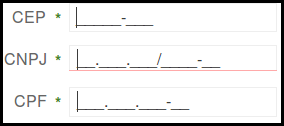
\includegraphics[width=8cm]{mascara}
\caption{Máscaras de entrada: CEP, CNPJ e CPF}
\label{figMascara}
\end{figure}

Figura~\ref{figMascara}  apresenta  um  exemplo  das  máscaras  de  entrada  dos
atributos  CEP, CNPJ  e CPF  da aplicação  {\bf ControleBancario}.  Na definição
dessas  máscaras de entrada,  foi utilizado  o {\it  plugin} {\bf  jQuery Masked
  Input}\footnote{\url{http://digitalbush.com/projects/masked-input-plugin/}}
que permite construir máscaras em campos HTML com as seguintes regras: 

\begin{itemize}

\vspace{0.3cm}

\item {\bf a} - Representa um caractere alfabético (A-Z, a-z)

\vspace{0.3cm}

\item {\bf 9} - Representa um digito (0-9)

\vspace{0.3cm}

\item {\bf *} - Representa um caractere alfanumérico (A-Z, a-z ,0-9)

\end{itemize}

\vspace{0.3cm}

Assim,  a máscara {\bf  999.999.999-99} define  um CPF  composto por  11 digitos
separados pelos caracteres: ponto ({\bf .}) e traço ({\bf -}).  

\vspace{0.3cm}

\begin{remark}
Análogo ao  {\bf create.gsp}, o  {\it template} {\bf edit.gsp}  também necessita
ser alterado para  definir as máscaras de entrada para os  atributos CEP, CNPJ e
CPF das classes  de domínio.  Então, fica como exercício  para o leitor realizar
tal alteração.
\end{remark}

\begin{lstlisting}[numbers=left,        caption={\it        Template}       {\bf
      scaffolding/create.gsp}, frame = trBL,float=htbp, label=codTemCreate] 
<!DOCTYPE html>
<html>
 <head>
  <meta name="layout" content="main">
  <g:set var="entityName" value="\${message(code: '${domainClass.propertyName}.label', 
                                             default: '${className}')}" />
  <title><g:message code="default.create.label" args="[entityName]" /></title>
  <g:javascript src="jquery-1.8.3.min.js"/>
  <g:javascript src="jquery.maskedinput.min.js"/> 
  <g:javascript>
   var JQuery = jQuery.noConflict()
   JQuery(document).ready(function(){
       JQuery("#CPF").mask("999.999.999-99");
       JQuery("#CNPJ").mask("99.999.999/9999-99");
       JQuery("#CEP").mask("99999-999");
   });
  </g:javascript>
 </head>
 <body>
  <a href="#create-${domainClass.propertyName}" class="skip" tabindex="-1">
  <g:message code="default.link.skip.label" default="Skip to content&hellip;"/></a>
  <div class="nav" role="navigation">
   <ul>
    <li><a class="home" href="\${createLink(uri: '/')}"><g:message code="default.home.label"/></a></li>
    <li><g:link class="list" action="index"><g:message code="default.list.label" args="[entityName]"/>
        </g:link></li>
   </ul>
  </div>
  <div id="create-${domainClass.propertyName}" class="content scaffold-create" role="main">
   <h1><g:message code="default.create.label" args="[entityName]" /></h1>
   <g:if test="\${flash.message}">
    <div class="message" role="status">\${flash.message}</div>
   </g:if>
   <g:hasErrors bean="\${${propertyName}}">
    <ul class="errors" role="alert">
     <g:eachError bean="\${${propertyName}}" var="error">
      <li <g:if test="\${error in org.springframework.validation.FieldError}">data-field-id="\${error.field}"
          </g:if>>
      <g:message error="\${error}"/></li>
     </g:eachError>
    </ul>
   </g:hasErrors>
   <g:form url="[resource:${propertyName}, action:'save']" 
    <%= multiPart ? ' enctype="multipart/form-data"' : '' %>>
    <fieldset class="form">
     <g:render template="form"/>
    </fieldset>
    <fieldset class="buttons">
     <g:submitButton name="create" class="save" value="\${message(code: 'default.button.create.label', 
                                                                  default: 'Create')}" />
    </fieldset>
   <g:form>
  </div>
 </body>
</html>
\end{lstlisting}

\subsection{Template: index.gsp}

\vspace{0.5cm}

O {\it template}  {\bf index.gsp} é utilizado na geração  das visões {\bf index}
associadas a cada  um dos controladores da aplicação.   No contexto da aplicação
{\bf     ControleBancario},     esse     {\it    template}     será     alterado
(Código~\ref{codTemIndex}, linhas  17-20) de tal forma  que o {\it  link} para a
operação de criação  de entidades (ação {\bf create()})  apenas será apresentada
se o  usuário encontra-se  autenticado e possui  papel necessário  para executar
essa ação.

O {\it plugin} {\bf spring-security} define algumas {\it tags} GSP que permite a
exibição  condicional de {\it  links} de  acesso a  ações de  controladores.  Ou
seja,  aquele {\it  link} apenas  será  apresentado em  uma visão  se o  usuário
encontra-se autenticado e possui papel necessário para executar a ação.
\index{Plugins!spring-security} 

Por exemplo, a {\it tag}  GSP {\bf <sec: ifLoggedin>} apresentada abaixo, apenas
renderizaria a mensagem {\em Bemvindo!}, se o usuário encontra-se autenticado.

\vspace{0.3cm}

\begin{cBox}
\begin{footnotesize}
\begin{verbatim}
<sec:ifLoggedIn>
Bemvindo!
</sec:ifLoggedIn>
\end{verbatim}
\end{footnotesize}
\end{cBox}

\vspace{0.3cm}

Como  outro  exemplo,  a  {\it  tag}  GSP {\bf  <sec:  access>}  abaixo,  apenas
renderizaria  o  {\it  link}  para  a  ação {\bf  create}  do  controlador  {\bf
  transacao},  se o usuário  encontra-se autenticado  e possui  papel necessário
para executar a ação.  

\vspace{0.3cm}

\begin{cBox}
\begin{footnotesize}
\begin{verbatim}
<sec:access controller='transacao' action='create'>
   <g:link controller='transacao' action='create'>Cria Transação</g:link>
</sec:access>
\end{verbatim}
\end{footnotesize}
\end{cBox}

\vspace{0.3cm}

Para maiores  informações sobre as {\it  tags} GSP, definidas  pelo {\it plugin}
{\bf   spring-security},  o   leitor   pode  consultar   o  seguinte   endereço:
\url{http://grails.org/plugin/spring-security-core}. 

\begin{lstlisting}[numbers=left,        caption={\it        Template}       {\bf
      scaffolding/index.gsp}, frame = trBL,float=htbp, label=codTemIndex] 
<% import grails.persistence.Event %>
<%=packageName%>
<!DOCTYPE html>
<html>
   <head>
    <meta name="layout" content="main">
    <g:set var="entityName" value="\${message(code:'${domainClass.propertyName}.label',default:'${className}')}" />
    <title><g:message code="default.list.label" args="[entityName]" /></title>
   </head>
   <body>
     <a href="#list-${domainClass.propertyName}" class="skip" tabindex="-1">
     <g:message code="default.link.skip.label" default="Skip to content&hellip;"/></a>
      <div class="nav" role="navigation">
       <ul>
        <li><a class="home" href="\${createLink(uri: '/')}"><g:message code="default.home.label"/></a></li>
        <li>
          <sec:access controller="${domainClass.propertyName}" action='create'>
            <g:link class="create" action="create"><g:message code="default.new.label" args="[entityName]" />
            </g:link>
          </sec:access>
         </li> 
       </ul>
       </div>
       <div id="list-${domainClass.propertyName}" class="content scaffold-list" role="main">
         <h1><g:message code="default.list.label" args="[entityName]" /></h1>
          <g:if test="\${flash.message}">
            <div class="message" role="status">\${flash.message}</div>
          </g:if>
          <table>
           <thead>
             <tr>
              <% excludedProps = Event.allEvents.toList() << 'id' << 'version'
                 allowedNames = domainClass.persistentProperties*.name << 'dateCreated' << 'lastUpdated'
                 props = domainClass.properties.findAll { allowedNames.contains(it.name) && 
                 !excludedProps.contains(it.name) && it.type != null && !Collection.isAssignableFrom(it.type) }
                 Collections.sort(props, comparator.constructors[0].newInstance([domainClass] as Object[]))
                 props.eachWithIndex { p, i ->
                 if (i < 6) {
                  if (p.isAssociation()) { %>
              <th><g:message code="${domainClass.propertyName}.${p.name}.label" default="${p.naturalName}" /></th>
               <%      } else { %>
               <g:sortableColumn property="${p.name}" title="\${message(code:'${domainClass.propertyName}.
               ${p.name}.label', default: '${p.naturalName}')}" />
               <%  }   }   } %>
            </tr>
           </thead>
           <tbody>
            <g:each in="\${${propertyName}List}" status="i" var="${propertyName}">
             <tr class="\${(i % 2) == 0 ? 'even' : 'odd'}">
             <%  props.eachWithIndex { p, i ->
             if (i == 0) { %>
              <td><g:link action="show" id="\${${propertyName}.id}">\${fieldValue(bean: ${propertyName}, 
                  field: "${p.name}")}</g:link></td>
              <%      } else if (i < 6) {
              if (p.type == Boolean || p.type == boolean) { %>
              <td><g:formatBoolean boolean="\${${propertyName}.${p.name}}" /></td>
              <% } else if (p.type==Date||p.type==java.sql.Date||p.type==java.sql.Time||p.type==Calendar) { %>
              <td><g:formatDate date="\${${propertyName}.${p.name}}" /></td>
              <%          } else { %>
              <td>\${fieldValue(bean: ${propertyName}, field: "${p.name}")}</td>
              <%  }   }   } %>
             </tr>
            </g:each>
           </tbody>
          </table>
          <div class="pagination">
           <g:paginate total="\${${propertyName}Count ?: 0}" />
          </div>
       </div>
   </body>
</html>
\end{lstlisting}

\subsection{Template: show.gsp}

\vspace{0.5cm}

O {\it  template} {\bf show.gsp}  é utilizado na  geração das visões  {\bf show}
associadas a cada  um dos controladores da aplicação.   No contexto da aplicação
{\bf  ControleBancario}, esse  {\it  template} será  alterado  para refletir  as
seguintes funcionalidades:

\vspace{0.3cm}

\begin{itemize}

\item O {\it link} para a operação de criação de entidades (ação {\bf create()})
  apenas será  apresentada se o  usuário encontra-se autenticado e  possui papel
  necessário para executar essa ação (Código~\ref{codTemShow}, linhas 17-20).

\vspace{0.3cm}

\item  O botão {\bf  edit}, responsável  pela edição  de entidades,  apenas será
  apresentada  se o usuário  encontra-se autenticado  e possui  papel necessário
  para executar essa ação (Código~\ref{codTemShow}, linhas 68-71).  

\vspace{0.3cm}
 
\item O botão  {\bf delete}, responsável pela remoção  de entidades, apenas será
  apresentada  se o usuário  encontra-se autenticado  e possui  papel necessário
  para executar essa ação (Código~\ref{codTemShow}, linhas 72-76).

\end{itemize}

\begin{lstlisting}[numbers=left,        caption={\it        Template}       {\bf
      scaffolding/show.gsp}, frame = trBL,float=htbp, label=codTemShow] 
<% import grails.persistence.Event %>
<%=packageName%>
<!DOCTYPE html>
<html>
  <head>
    <meta name="layout" content="main">
    <g:set var="entityName" value="\${message(code:'${domainClass.propertyName}.label',default:'${className}')}"/>
    <title><g:message code="default.show.label" args="[entityName]" /></title>
  </head>
  <body>
    <a href="#show-${domainClass.propertyName}" class="skip" tabindex="-1"><g:message 
                     code="default.link.skip.label" default="Skip to content&hellip;"/></a>
    <div class="nav" role="navigation">
     <ul>
      <li><a class="home" href="\${createLink(uri: '/')}"><g:message code="default.home.label"/></a></li>
      <li><g:link class="list" action="index"><g:message code="default.list.label" args="[entityName]"/></g:link>
      </li><li>
       <sec:access controller="${domainClass.propertyName}" action='create'>
        <g:link class="create" action="create"><g:message code="default.new.label" args="[entityName]" /></g:link>
       </sec:access>
      </li>
     </ul>
    </div>
    <div id="show-${domainClass.propertyName}" class="content scaffold-show" role="main">
     <h1><g:message code="default.show.label" args="[entityName]" /></h1>
     <g:if test="\${flash.message}">
      <div class="message" role="status">\${flash.message}</div>
     </g:if>
     <ol class="property-list ${domainClass.propertyName}">
     <%  excludedProps = Event.allEvents.toList() << 'id' << 'version'
allowedNames = domainClass.persistentProperties*.name << 'dateCreated' << 'lastUpdated'
props = domainClass.properties.findAll { allowedNames.contains(it.name) && !excludedProps.contains(it.name) }
Collections.sort(props, comparator.constructors[0].newInstance([domainClass] as Object[]))
props.each { p -> %>
     <g:if test="\${${propertyName}?.${p.name}}">
      <li class="fieldcontain">
       <span id="${p.name}-label" class="property-label"><g:message 
             code="${domainClass.propertyName}.${p.name}.label" default="${p.naturalName}" /></span>
       <%  if (p.isEnum()) { %>
       <span class="property-value" aria-labelledby="${p.name}-label">
       <g:fieldValue bean="\${${propertyName}}" field="${p.name}"/></span>
       <%  } else if (p.oneToMany || p.manyToMany) { %>
       <g:each in="\${${propertyName}.${p.name}}" var="${p.name[0]}">
        <span class="property-value" aria-labelledby="${p.name}-label">
        <g:link controller="${p.referencedDomainClass?.propertyName}" action="show" id="\${${p.name[0]}.id}">
          \${${p.name[0]}?.encodeAsHTML()}</g:link></span>
       </g:each>
       <%  } else if (p.manyToOne || p.oneToOne) { %>
       <span class="property-value" aria-labelledby="${p.name}-label">
       <g:link controller="${p.referencedDomainClass?.propertyName}" action="show" 
       id="\${${propertyName}?.${p.name}?.id}">\${${propertyName}?.${p.name}?.encodeAsHTML()}</g:link></span>
       <%  } else if (p.type == Boolean || p.type == boolean) { %>
       <span class="property-value" aria-labelledby="${p.name}-label">
       <g:formatBoolean boolean="\${${propertyName}?.${p.name}}" /></span>
       <% } else if (p.type==Date || p.type==java.sql.Date || p.type==java.sql.Time || p.type==Calendar) { %>
       <span class="property-value" aria-labelledby="${p.name}-label">
       <g:formatDate date="\${${propertyName}?.${p.name}}" /></span>
       <%  } else if (!p.type.isArray()) { %>
       <span class="property-value" aria-labelledby="${p.name}-label">
       <g:fieldValue bean="\${${propertyName}}" field="${p.name}"/></span>
       <%  } %>
      </li>
     </g:if>
     <%  } %>
    </ol>
    <g:form url="[resource:${propertyName}, action:'delete']" method="DELETE">
     <fieldset class="buttons">
      <sec:access controller="${domainClass.propertyName}" action='edit'>
       <g:link class="edit" action="edit" resource="\${${propertyName}}">
       <g:message code="default.button.edit.label" default="Edit" /></g:link>
      </sec:access>
      <sec:access controller="${domainClass.propertyName}" action='delete'>
       <g:actionSubmit class="delete" action="delete" value="\${message(code: 'default.button.delete.label', 
       default: 'Delete')}" onclick="return confirm('\${message(code: 'default.button.delete.confirm.message', 
       default: 'Are you sure?')}');" />
      </sec:access>
     </fieldset>
    </g:form>
   </div>
  </body>
</html>
\end{lstlisting}

\newpage

\section{Controladores e Visões}

Após realizar as alterações discutidas  na seção anterior, é necessário executar
o  comando  {\bf generate-all}  para  que  as  alterações nos  {\it  templates},
discutidos na  seção anterior,  sejam refletidos nos  controladores e  visões da
aplicação  {\bf ControleBancario}.  No  IDE GGTS:  Selecione {\bf  Grails Tools}
$\Longrightarrow$ {\bf Grails Command Wizard}.  Digite {\bf generate-all} como o
nome do comando a ser executado e clique em {\bf Next}.  Digite o nome da classe
de    domínio   como    o   parâmetro    do   comando    e   clique    em   {\bf
  Next}.  Tabela~\ref{tblGenerateAll} lista o  nome das  classes de  domínio que
necessitam que os controladores e visões sejam geradas novamente.
\index{Comandos!grails generate-all} 

\begin{table}[htbp]
\centering
\begin{tabular}{|c|c|c|c|c|}
\hline
\rowcolor{Gray}
Agencia & Banco & CaixaEletronico & Cidade & ClienteFisico \\ \hline
\rowcolor{C2}
ClienteJuridico & ContaCliente & ContaCorrente & ContaPoupanca & Endereco \\ \hline
\rowcolor{Gray}
Estado & Gerente &Transacao & &\\ \hline
\end{tabular}
\caption{Classes de domínio: geração dos Controladores e Visões.}
\label{tblGenerateAll}
\end{table}

\subsection{Controlador: ContaController}

\vspace{0.5cm}

O  próximo passo  consiste na  definição  do {\bf  ContaController} associado  à
classe  de  domínio {\bf  Conta}.   Esse  controlador  implementa operações  que
uniformiza o acesso às instâncias das subclasses da classe abstrata {\bf Conta}.
Por exemplo, a ação {\bf index()} é responsável por listar contas bancárias (não
importando se elas são contas correntes ou contas poupanças).

Para criar um  controlador, relacionado à classe de domínio  {\bf Conta}, no IDE
GGTS:   Selecione    {\bf   Grails   Tools}    $\Longrightarrow$   {\bf   Create
  Controller}.  Digite {\bf br.ufscar.dc.dsw.Conta} como o nome do controlador e
clique em {\bf Finish}. Abra  o controlador {\bf ContaController} e implemente-o
conforme apresentado no Código~\ref{codContaController}. 

\begin{lstlisting}[caption=Controlador    {\bf    ContaController},   frame    =
    trBL,float=htbp, label=codContaController] 
package br.ufscar.dc.dsw

import static org.springframework.http.HttpStatus.*
import grails.transaction.Transactional
import org.springframework.security.access.annotation.Secured

@Secured('ROLE_GERENTE')
class ContaController {
    
    static allowedMethods = [save: "POST", update: "PUT", delete: "DELETE"]
    
    def index(Integer max) {
        params.max = Math.min(max ?: 10, 100)
        respond Conta.list(params), model:[list: Conta.list(params), contaInstanceCount: Conta.count()]
    }
    
    @Secured(['ROLE_ADMIN', 'ROLE_CLIENTE', 'ROLE_GERENTE'])
    def show() {
        Conta instance = Conta.get(params.id)
        if (instance.instanceOf(ContaCorrente)) {
            forward controller: 'contaCorrente', action: "show"
        } else {
            forward controller: 'contaPoupanca', action: "show"
        }
    }
}

\end{lstlisting}

\begin{itemize}

\item A ação {\bf index()} é  restrita aos usuários que desempenham o papel {\bf
  ROLE\_GERENTE}; e 

\vspace{0,3cm}

\item A  ação {\bf show()}  é restrita aos  usuários que desempenham  os papéis:
  {\bf ROLE\_ADMIN}, {\bf ROLE\_CLIENTE} e {\bf ROLE\_GERENTE}. Além disso, essa
  ação  verifica  se a  instância  é  uma conta  corrente  ou  conta poupança  e
  direciona para o controlador mais apropriado: {\bf ContaCorrenteController} ou
  {\bf ContaPoupancaController}.  

\end{itemize}

\subsection{Visão: conta/index.gsp}

\vspace{0.5cm}

Relembrando   a   discussão  da   Seção~\ref{secEstatico},   para  cada   método
correspondente a  uma ação em um  controlador é criada  uma correspondente visão
(arquivo  com  extensão  {\bf  .gsp}).  Assim,  a  ação  {\bf  index},  de  {\bf
  ContaController}, tem o correspondente {\bf index.gsp}.  

\vspace{0.2cm}

A visão {\bf index.gsp} apresenta  uma lista de contas bancárias (não importando
se elas são  contas correntes ou contas poupanças).  A implementação dessa visão
encontra-se apresentada no Código~\ref{codContaIndex}. 

\vspace{0.3cm}

\begin{lstlisting}[numbers=left,     caption=Visão     {\bf    conta/index.gsp},
    frame=trBL,float=htbp, label=codContaIndex] 
<%@ page import="br.ufscar.dc.dsw.Conta" %>
<!DOCTYPE html>
<html>
 <head>
  <meta name="layout" content="main">
  <g:set var="entityName" value="${message(code: 'conta.label', default: 'Conta')}" />
  <title><g:message code="default.list.label" args="[entityName]" /></title>
 </head>
 <body>
  <a href="#list-conta" class="skip" tabindex="-1"><g:message code="default.link.skip.label" 
     default="Skip to content&hellip;"/></a>
  <div class="nav" role="navigation">
   <ul>
    <li>
     <a class="home" href="${createLink(uri: '/')}"><g:message code="default.home.label"/></a>
    </li>
   </ul>
  </div>
  <div id="list-conta" class="content scaffold-list" role="main">
   <h1><g:message code="default.list.label" args="[entityName]" /></h1>
   <g:if test="${flash.message}">
    <div class="message" role="status">${flash.message}</div>
   </g:if>
   <table>
    <thead>
     <tr>
      <g:sortableColumn property="numero" title="${message(code: 'conta.numero.label', default: 'Numero')}" />
      <th>
        <g:message code="conta.agencia.label" default="Agencia" />
      </th>
      <g:sortableColumn property="saldo" title="${message(code: 'conta.saldo.label', default: 'Saldo')}" />
      <g:sortableColumn property="abertura" title="${message(code:'conta.abertura.label',default:'Abertura')}" />
     </tr>
    </thead>
    <tbody>
     <g:each in="${list}" status="i" var="contaInstance">
      <tr class="${(i % 2) == 0 ? 'even' : 'odd'}">
       <td>
         <g:link action="show" id="${contaInstance.id}">${fieldValue(bean: contaInstance, field: "numero")}
         </g:link>
       </td>
       <td>${fieldValue(bean: contaInstance, field: "agencia")}</td>
       <td>${fieldValue(bean: contaInstance, field: "saldo")}</td>
       <td><g:formatDate date="${contaInstance.abertura}" /></td>
      </tr>
     </g:each>
    </tbody>
   </table>
   <div class="pagination">
    <g:paginate total="${contaInstanceCount ?: 0}" />
   </div>
  </div>
 </body>
</html>
\end{lstlisting}

\vspace{0.3cm}

\noindent Conforme pode-se observar, essa  visão constrói uma tabela HTML com os
atributos  (número, agência,  saldo e  data  de abertura)  das contas  bancárias
retornadas.   É importante  salientar  que  é através  da  variável {\bf  list},
retornada pela  ação {\bf index()},  que essa visão  tem acesso aos  valores dos
atributos das contas bancárias.  

\newpage

\subsection{Controlador: ClienteController}

\vspace{0.5cm}

Análogo ao {\bf ContaControlador}, o {\bf ClienteController}, associado à classe
de  domínio {\bf  Cliente},  implementa  operações que  uniformiza  o acesso  às
instâncias das subclasses da classe abstrata {\bf Cliente}.  Por exemplo, a ação
{\bf  index()} é responsável  por listar  clientes (não  importando se  eles são
clientes físicos ou jurídicos). 

\vspace{0.3cm}

Para criar um controlador, relacionado à classe de domínio {\bf Cliente}, no IDE
GGTS:   Selecione    {\bf   Grails   Tools}    $\Longrightarrow$   {\bf   Create
  Controller}.  Digite {\bf br.ufscar.dc.dsw.Cliente} como o nome do controlador
e  clique  em  {\bf  Finish}.   Abra o  controlador  {\bf  ClienteController}  e
implemente-o conforme apresentado no Código~\ref{codClienteController}.  


\begin{lstlisting}[caption=Controlador          {\bf         ClienteController},
    frame=trBL,float=htbp, label=codClienteController] 
package br.ufscar.dc.dsw

import static org.springframework.http.HttpStatus.*
import grails.transaction.Transactional
import org.springframework.security.access.annotation.Secured

@Secured('ROLE_GERENTE')
class ClienteController {
    
    static allowedMethods = [save: "POST", update: "PUT", delete: "DELETE"]
    def index(Integer max) {
        params.max = Math.min(max ?: 10, 100)
        respond Cliente.list(params), model:[list: Cliente.list(params), clienteInstanceCount: Cliente.count()]
    }
    
    @Secured(['ROLE_ADMIN', 'ROLE_CLIENTE', 'ROLE_GERENTE'])
    def show() {
        Cliente instance = Cliente.get(params.id)
        if (instance.instanceOf(ClienteFisico)) {
            forward controller: 'clienteFisico', action: "show"
        } else {
            forward controller: 'clienteJuridico', action: "show"
        }
    }
}
\end{lstlisting}

\begin{itemize}

\item A ação {\bf index()} é  restrita aos usuários que desempenham o papel {\bf
  ROLE\_GERENTE}; e 

\vspace{0,3cm}

\item A ação {\bf show()} é restrita aos usuários que desempenham os respectivos
  papéis:  {\bf ROLE\_ADMIN},  {\bf ROLE\_CLIENTE}  e {\bf  ROLE\_GERENTE}. Além
  disso,  essa ação  verifica se  a  instância é  um cliente  físico ou  cliente
  jurídico   e   direciona   para    o   controlador   mais   apropriado:   {\bf
    ClienteFisicoController} ou {\bf ClienteJuridicoController}.  

\end{itemize}

\vspace{0.3cm}

\subsection{Visão: cliente/index.gsp}

\vspace{0.5cm}

A visão {\bf index.gsp} apresenta uma  lista de clientes (não importando se eles
são  clientes físicos ou  jurídicos).  A  implementação dessa  visão encontra-se
apresentada no Código~\ref{codCliIndex}. 

\vspace{0.3cm}

\begin{itemize}

\item  Conforme pode-se observar,  essa visão  constrói uma  tabela HTML  com os
  atributos (nome, endereço, data de  moradia e status) dos clientes retornados.
  É importante  salientar que é através  da variável {\bf  list}, retornada pela
  ação {\bf  index()}, que essa visão  tem acesso aos valores  dos atributos dos
  clientes.  

\end{itemize}

\newpage

\begin{lstlisting}[caption=Visão       {\bf       cliente/index.gsp},      frame
    =trBL,float=htbp, label=codCliIndex] 
<%@ page import="br.ufscar.dc.dsw.Cliente" %>
<!DOCTYPE html>
<html>
  <head>
   <meta name="layout" content="main">
   <g:set var="entityName" value="${message(code: 'cliente.label', default: 'Cliente')}" />
   <title><g:message code="default.list.label" args="[entityName]" /></title>
  </head>
  <body>
   <a href="#list-cliente" class="skip" tabindex="-1"><g:message code="default.link.skip.label" default="Skip to content&hellip;"/></a>
    <div class="nav" role="navigation">
     <ul>
      <li><a class="home" href="${createLink(uri: '/')}"><g:message code="default.home.label"/></a></li>
     </ul>
    </div>
    <div id="list-cliente" class="content scaffold-list" role="main">
     <h1><g:message code="default.list.label" args="[entityName]" /></h1>
      <g:if test="${flash.message}">
       <div class="message" role="status">${flash.message}</div>
      </g:if>
      <table>
       <thead>
        <tr>
         <g:sortableColumn property="nome" title="${message(code: 'cliente.nome.label', default: 'Nome')}" />
         <th><g:message code="cliente.endereco.label" default="Endereco" /></th>
         <g:sortableColumn property="dtMoradia" title="${message(code: 'cliente.dtMoradia.label', default: 'Dt Moradia')}" />
         <g:sortableColumn property="status" title="${message(code: 'cliente.status.label', default: 'Status')}" />
        </tr>
       </thead>
       <tbody>
        <g:each in="${list}" status="i" var="clienteInstance">
         <tr class="${(i % 2) == 0 ? 'even' : 'odd'}">
          <td><g:link action="show" id="${clienteInstance.id}">${fieldValue(bean: clienteInstance, field: "nome")}</g:link></td>
          <td>${fieldValue(bean: clienteInstance, field: "endereco")}</td>
          <td><g:formatDate date="${clienteInstance.dtMoradia}" /></td>
          <td>${fieldValue(bean: clienteInstance, field: "status")}</td>
         </tr>
        </g:each>
       </tbody>
      </table>
      <div class="pagination">
       <g:paginate total="${clienteInstanceCount ?: 0}" />
      </div>
     </div>
   </body>
</html>
\end{lstlisting}

\subsection{Mapeamento URL}\index{URL!Mapeamento}

\vspace{0.3cm}

Pela convenção, ao executar a aplicação,  a página principal é a que lista todos
os  controladores  da  aplicação.   Porém  é possível  alterar  o  arquivo  {\bf
  conf/URLMapping.groovy}      para      definir     outro      controlador/ação
padrão. Código~\ref{codURLMappings} define, como a página principal, a ação {\bf
  index()} do controlador {\bf MainController} (Seção~\ref{secMainController}).  

\begin{lstlisting}[caption={\bf   URLMappings.groovy},  frame=trBL,  float=htbp,
    label=codURLMappings] 
class UrlMappings {
	static mappings = {
        "/$controller/$action?/$id?(.$format)?"{
            constraints {
                // apply constraints here
            }
        }
        "/"(controller:"main")
        "500"(view:'/error')
	}
}
\end{lstlisting}

\newpage

\subsection{Controlador: MainController}\label{secMainController}

\vspace{0.5cm}

O  {\bf MainController}  consiste  no controlador  principal  da aplicação  {\bf
  ControleBancario}.   Para criar um  controlador, no  IDE GGTS:  Selecione {\bf
  Grails  Tools}   $\Longrightarrow$  {\bf  Create   Controller}.   Digite  {\bf
  br.ufscar.dc.dsw.Main} como  o nome do  controlador e clique em  {\bf Finish}.
Abra o  controlador {\bf MainController} e implemente-o  conforme apresentado no
Código~\ref{codMainController}.  

\begin{lstlisting}[caption=Controlador    {\bf    MainController},   frame=trBL,
    float=htbp, label=codMainController] 
package br.ufscar.dc.dsw

import org.springframework.security.access.annotation.Secured

@Secured(['ROLE_ADMIN', 'ROLE_CLIENTE', 'ROLE_GERENTE'])
class MainController {

    def index() { }
}
\end{lstlisting}

\begin{itemize}

\item  A  ação  {\bf  index()}  é  restrita  aos  usuários  que  desempenham  os
  respectivos   papéis:   {\bf   ROLE\_ADMIN},   {\bf  ROLE\_CLIENTE}   e   {\bf
    ROLE\_GERENTE}.  

\end{itemize}

\subsection{Visão: main/index.gsp}

\vspace{0.5cm}

A  visão {\bf  main/index.gsp} consiste  na  visão principal  da aplicação  {\bf
  ControleBancario}.   A implementação  dessa visão  encontra-se  apresentada no
Código~\ref{codMainIndex}.  

\lstset{language=XML}
\begin{lstlisting}[numbers=left, caption=Visão {\bf main/index.gsp}, frame=trBL,
    float=htbp, label=codMainIndex] 
<!DOCTYPE html>
<html>
 <head>
  <meta name="layout" content="main">
  <g:javascript library="jquery" />
 </head>
 <body>
  <div id="status" role="complementary">
   <h1>Op^çõ^es</h1>
   <table>
    <g:each var="c" in="${grailsApplication.controllerClasses.sort { it.fullName } }">
     <g:set var="name" value="${c.logicalPropertyName}" />
     <g:if test="${name != 'logout' && name != 'login' && name != 'main'}">
      <sec:access url='${createLink(controller: c.logicalPropertyName, base: "/")}'>
       <tr><td>    
        <g:link controller="${c.logicalPropertyName}">${c.naturalName.replace(" Controller","")}</g:link>
       </td></tr>
      </sec:access>
     </g:if>
    </g:each>
   </table>
  </div>
 </body>
</html>
\end{lstlisting}

Pode-se  observar,  pelas  linhas  14-18,   que  a  visão  apenas  apresenta  os
controladores para qual o usuário autenticado tem permissão de acessá-lo. Assim,
para  os usuários  que  desempenham  diferentes papéis,  a  página principal  da
aplicação {\bf ControleBancario} torna-se diferente. 

\vspace{0.2cm}

Figura~\ref{figVisao}(a) apresenta  a página principal conforme  acessada por um
usuário    que     desempenha    o    papel     {\bf    ROLE\_ADMIN}    enquanto
Figura~\ref{figVisao}(b)  apresenta  a página  principal  conforme acessada  por
usuário que desempenha o papel {\bf ROLE\_GERENTE}.  

\newpage

\begin{figure}[htbp]
\center
\subfigure[Visão: Papel Administrador]{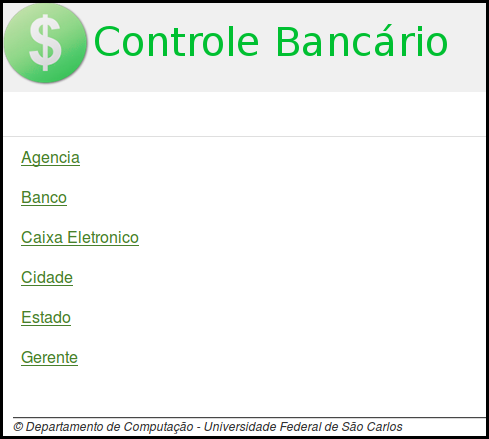
\includegraphics[height=6.5cm]{VisaoAdmin}}
\qquad
\subfigure[Visão: Papel Gerente]{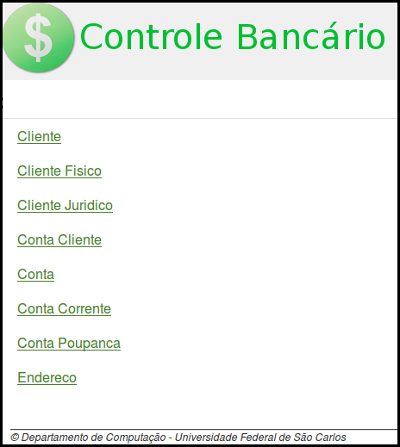
\includegraphics[height=6.5cm]{VisaoGerente}}
\caption{Visão main/index.gsp: diferentes visões}
\label{figVisao}
\end{figure}

\subsection{Controladores: últimas alterações relacionadas ao controle de acesso}

\vspace{0.3cm}

Por  fim, atualize os  controladores conforme  o Código~\ref{codControleAcesso}.
Pelo código, observa-se que: 

\vspace{0.3cm}

\begin{itemize}

\item      Os     controladores     {\bf      ClienteFisicoController},     {\bf
  ClienteJuridicoController},       {\bf      ContaClienteController},      {\bf
  ContaCorrenteController},     {\bf     ContaPoupancaController}     e     {\bf
  EnderecoController}  serão apenas  acessados  por usuários  que desempenham  o
  papel de gerente; e 

\vspace{0.3cm}

\item O controlador {\bf  TransacaoController} será apenas acessado por usuários
  que desempenham o papel de cliente.

\end{itemize}

\begin{lstlisting}[caption=Controladores  - últimas  alterações  relacionadas ao
    Controle de Acesso, frame = trBL,float=htbp, label=codControleAcesso] 
@Secured('ROLE_GERENTE')
class ClienteFisicoController {
  // Implementa^çã^o do controlador ClienteFisico
}

@Secured('ROLE_GERENTE')
class ClienteJuridicoController {
  // Implementa^çã^o do controlador ClienteJuridico
}

@Secured('ROLE_GERENTE')
class ContaClienteController {
  // Implementa^çã^o do controlador ClienteCliente
}

@Secured('ROLE_GERENTE')
class ContaCorrenteController {
  // Implementa^çã^o do controlador ContaCorrente
}

@Secured('ROLE_GERENTE')
class ContaPoupancaController {
  // Implementa^çã^o do controlador ContaPoupanca
}

@Secured('ROLE_GERENTE')
class EnderecoController {
  // Implementa^çã^o do controlador Endereco
}

@Secured('ROLE_CLIENTE')
class TransacaoController {
  // Implementa^çã^o do controlador Transacao
}
\end{lstlisting}

\newpage

\section{Melhorando o leiaute da aplicação: biblioteca de marca}

\vspace{0.3cm}

Com  o objetivo  de melhorar  o  leiaute da  aplicação, essa  seção apresenta  a
implementação de uma biblioteca de marca ({\it taglib}) que é utilizada em todas
as visões da aplicação {\bf ControleBancario}. Os passos são descritos a seguir: 

\begin{itemize}

\vspace{0.3cm}

\item Para  criar uma biblioteca  de marca, no  IDE GGTS: Selecione  {\bf Grails
  Tools} $\Longrightarrow$ {\bf Create TagLib}.   Digite {\bf Login} como o nome
  da biblioteca de  marca e clique em {\bf Finish}. Abra  a biblioteca de marcas
  {\bf     LoginTagLib}    e     implemente-o     conforme    apresentado     no
  Código~\ref{codTagLib}.  Pelo código-fonte, observa-se que essa classe imprime
  o nome do papel desempenhado pelo usuário {\it logado}.  

\begin{lstlisting}[caption=Biblioteca  de marca  {\bf  LoginTagLib}, frame=trBL,
    float=htbp, label=codTagLib] 
class LoginTagLib {
    def springSecurityService
    def loginControl = {
        if (springSecurityService.isLoggedIn()) {
            def usuario = springSecurityService.getCurrentUser() 
            def authority = usuario.getAuthorities()[0].getAuthority()
            def papel
            if (authority.equals('ROLE_ADMIN')) {
                papel = "Administrador"
            } else if (authority.equals('ROLE_CLIENTE')) {
                papel = "Cliente"
            } else {
                papel = "Gerente"
            }
            out << "<span style=\"padding-right:50px\">" << papel << "</span>"
            out << "<span style=\"padding-right:25px\">"
            out << """ [${link(controller: "logout"){"Logout"}}]"""
            out << "</span>"
        }
    }
}
\end{lstlisting}

\item Inclua o  {\it template} \_footer (grails-app/views/layouts/\_footer.gsp)
  com o  conteúdo apresentado  na Listagem~\ref{footerLst}. Esse  {\it template}
  será o rodapé presente em todas as visões da aplicação.

\lstset{language=XML}
\begin{lstlisting}[caption={\it   Template}   {\bf  \_footer.gsp},   frame=trBL,
    float=htbp, label=footerLst] 
<div id="footer">
 <hr/> &copy; DC - UFSCar
</div>
\end{lstlisting}

\item Incluir o  {\it template} \_header (grails-app/views/layouts/\_header.gsp)
  com o  conteúdo apresentado  na Listagem~\ref{headerLst}. Esse  {\it template}
  será o cabeçalho presente em todas as visões da aplicação. Observa-se que esse
  {\it  template} utiliza  a  biblioteca de  marcas  {\bf LoginTagLib}  definida
  anteriormente. 

\lstset{language=XML}
\begin{lstlisting}[caption={\it   Template}   {\bf  \_header.gsp},   frame=trBL,
    float=htbp, label=headerLst]
<div id="header">
 <p>
  <a class="header-main" href="${resource(dir:'')}">Contatos</a>
 </p>
 <div id = "loginHeader">
  <g:loginControl/>
 </div>
</div>
\end{lstlisting}

\newpage

\item    No     leaiute    padrão,    utilizado    por     todas    as    visões
  (arquivo  grails-app/views/layouts/main.gsp), realize  as  alterações conforme
  apresentadas pelo Código~\ref{codMain}.  Pelo código-fonte, observa-se que:

\begin{itemize}

\vspace{0.3cm}

\item A imagem de logo da aplicação é alterada (linha 23). É necessário realizar
  o    download     do    arquivo    {\bf     Controle.png},    disponível    em
  {\footnotesize\url{http://www.dc.ufscar.br/~delano/ControleBancario/Controle.png}}
  e copiá-lo no diretório {\bf web-app/images};

\vspace{0.3cm}

\item O {\it template} {\bf  header}, definido anteriormente, é utilizado (linha
  25); e 

\vspace{0.3cm}

\item O {\it template} {\bf  footer}, definido anteriormente, é utilizado (linha
  27). 

\end{itemize}

\lstset{language=XML}
\begin{lstlisting}[numbers=left,        caption=Leiaute        padrão       {\bf
      grails-app/views/layouts/main.gsp}, frame=trBL,float=htbp, label=codMain] 
<!DOCTYPE html>
 <!--[if lt IE 7 ]> <html lang="en" class="no-js ie6"> <![endif]-->
 <!--[if IE 7 ]> <html lang="en" class="no-js ie7"> <![endif]-->
 <!--[if IE 8 ]> <html lang="en" class="no-js ie8"> <![endif]-->
 <!--[if IE 9 ]> <html lang="en" class="no-js ie9"> <![endif]-->
 <!--[if (gt IE 9)|!(IE)]><!--> <html lang="en" class="no-js"><!--<![endif]-->
 <head>
  <meta http-equiv="Content-Type" content="text/html; charset=UTF-8">
  <meta http-equiv="X-UA-Compatible" content="IE=edge,chrome=1">
  <title><g:layoutTitle default="Controle Banc^á^rio"/></title>
  <meta name="viewport" content="width=device-width, initial-scale=1.0">
  <link rel="shortcut icon" href="${resource(dir: 'images', file: 'favicon.ico')}" type="image/x-icon">
  <link rel="apple-touch-icon" href="${resource(dir: 'images', file: 'apple-touch-icon.png')}">
  <link rel="apple-touch-icon" sizes="114x114" href="${resource(dir:'images',file:'apple-touch-icon-retina.png')}">
  <link rel="stylesheet" href="${resource(dir: 'css', file: 'main.css')}" type="text/css">
  <link rel="stylesheet" href="${resource(dir:'css',file:'mobile.css')}" type="text/css">
  <g:layoutHead/>
  <g:javascript library="application"/> 
  <r:layoutResources />
 </head>
 <body>
  <div id="grailsLogo" role="banner">
    <img src="${resource(dir: 'images', file: 'Controle.png')}" alt="Grails"/>
  </div>
  <g:render template="/layouts/header" />
  <g:layoutBody />
  <g:render template="/layouts/footer" />
  <div class="footer" role="contentinfo"></div>
  <div id="spinner" class="spinner" style="display:none;">
    <g:message code="spinner.alt" default="Loading&hellip;"/>
  </div>
  <r:layoutResources />
 </body>
</html>
\end{lstlisting}

\item Por fim, adicione as linhas no arquivo web-app/css/main.css conforme apresentado no Código~\ref{mainCSSLst}.

\lstset{language=XML}
\begin{lstlisting}[caption=Arquivo   {\bf   web-app/css/main.css},   frame=trBL,
    float=htbp, label=mainCSSLst] 
#grailsLogo {
	background-color: #f0f0f0;
}

#footer {
    font-size: 0.75em;
    font-style: italic;
    padding: 2em 1em 2em 1em;
    margin-bottom: 1em;
    margin-top: 1em;
    clear: both;
}

#loginHeader {
    float: right;
}
\end{lstlisting}

\end{itemize}

\section{Executando a aplicação}\label{secBootstrap2}

\vspace{0.3cm}

Conforme discutido anteriormente, antes  de executar a aplicação, instâncias das
entidades serão criadas.  No caso,  serão criados instâncias das entidades ({\bf
  Estado}, {\bf  Cidade}, {\bf Endereco}, etc) na  classe {\bf BootStrap.groovy}
que  encontra-se no  diretório {\bf  grails-app/conf}. Essa  classe  é executada
durante  o  {\it boot}  da  aplicação e  serve,  entre  outros propósitos,  para
inicializar a aplicação por exemplo, criando algumas instâncias de objetos. 

A   implementação   da  classe   {\bf   BootStrap.groovy}   é  apresentado   nos
Códigos~\ref{codBootStrap21}~a~\ref{codBootStrap25}.   O  trecho apresentado  no
Código~\ref{codBootStrap21},  popula  instâncias   das  classes  {\bf  Usuario},
{\bf Estado}  e {\bf  Cidade}. Observa-se  que o usuário  criado é  associado ao
papel  {\bf  ROLE\_ADMIN}. Ou  seja,  o usuário  criado  desempenha  o papel  de
administrador da aplicação {\bf ControleBancario}.  

\begin{lstlisting}[caption={\bf BootStrap.groovy (1)}, frame = trBL, float=htbp,
    label=codBootStrap21] 
import br.ufscar.dc.dsw.Agencia
import br.ufscar.dc.dsw.Banco
import br.ufscar.dc.dsw.CaixaEletronico
import br.ufscar.dc.dsw.Cidade
import br.ufscar.dc.dsw.Cliente
import br.ufscar.dc.dsw.ClienteFisico
import br.ufscar.dc.dsw.ClienteJuridico
import br.ufscar.dc.dsw.ContaCliente
import br.ufscar.dc.dsw.ContaCorrente
import br.ufscar.dc.dsw.ContaPoupanca
import br.ufscar.dc.dsw.Endereco
import br.ufscar.dc.dsw.Estado
import br.ufscar.dc.dsw.Gerente
import br.ufscar.dc.dsw.Papel
import br.ufscar.dc.dsw.Transacao
import br.ufscar.dc.dsw.Usuario
import br.ufscar.dc.dsw.UsuarioPapel

class BootStrap {
    def init = { servletContext ->
       
        def adminPapel = Papel.findByAuthority("ROLE_ADMIN") ?:
        new Papel(authority: "ROLE_ADMIN").save()
                
        def admin = new Usuario(
            username: "admin",
            password: "admin",
            nome: "Administrador",
            enabled : true
        )
        
        admin.save()
        if (admin.hasErrors()) {
            println admin.errors
        }
        UsuarioPapel.create(admin,adminPapel)
       
        print 'populando usu^á^rio admin - ok'
        
        def sp = new Estado(sigla: 'SP', nome: 'S^ã^o Paulo')
        
        sp.save()
        if (sp.hasErrors()) {
            println sp.errors
        }
        
        print 'populando estados - ok'
        
        def sanca = new Cidade(nome: 'S^ã^o Carlos', estado: sp)
        
        sanca.save()
        if (sanca.hasErrors()) {
            println sanca.errors
        }
        
        def sampa = new Cidade(nome: 'S^ã^o Paulo', estado: sp)
        
        sampa.save()
        if (sampa.hasErrors()) {
            println sampa.errors
        }
        
        print 'populando cidades - ok'
                        

\end{lstlisting}

\newpage

O  trecho  apresentado  no  Código~\ref{codBootStrap22}, popula  instâncias  das
classes {\bf Endereco}, {\bf Banco} e {\bf Agencia}.  

\begin{lstlisting}[caption={\bf BootStrap.groovy (2)}, frame = trBL, float=htbp,
    label=codBootStrap22] 
        def end1 = new Endereco(logradouro: 'R. Conde do Pinhal', numero: 1909, 
            bairro: 'Centro', CEP: '13560-648', cidade: sanca)

        end1.save()
        if (end1.hasErrors()) {
            println end1.errors
        }
        
        def end2 = new Endereco(logradouro: 'R. Treze de Maio', numero: 1930, 
            bairro: 'Centro', CEP: '13560-647', cidade: sanca)

        end2.save()
        if (end2.hasErrors()) {
            println end2.errors
        }
        
        def end3 = new Endereco(logradouro: 'R. Nilton Coelho de Andrade',
            numero: 772, bairro: 'Vila Maria', CEP:'03092-324', cidade: sampa)

        end3.save()
        if (end3.hasErrors()) {
            println end3.errors
        }
        
        def end4 = new Endereco(logradouro: 'R. Humberto Manelli', numero: 50, 
            complemento: 'Apto 31', bairro: 'Jardim Gibertoni', 
            CEP:'13562-420', cidade: sanca)
        end4.save()
        if (end4.hasErrors()) {
            println end4.errors
        }
        
        print 'populando endere^ç^os - ok'
        
        def bb = new Banco(numero: 1, nome: 'Banco do Brasil', 
            CNPJ: '00.000.000/0001-91')
        
        bb.save()
        if (bb.hasErrors()) {
            println bb.errors
        }
        
        def santander = new Banco(numero: 33, nome: 'Santander', 
            CNPJ: '90.400.888/0001-42')
        
        santander.save()
        if (santander.hasErrors()) {
            println santander.errors
        }

        print 'populando bancos - ok'
        
        def agencia1 = new Agencia(numero: 1888, nome: 'Conde do Pinhal', 
            endereco: end1, banco: bb)
        
        agencia1.save()
        if (agencia1.hasErrors()) {
            println agencia1.errors
        }
        
        def agencia2 = new Agencia(numero: 24, nome: 'Treze de Maio', 
            endereco: end2, banco: santander)
        
        agencia2.save()
        if (agencia2.hasErrors()) {
            println agencia2.errors
        }
        
        print 'populando ag^ê^ncias - ok'
\end{lstlisting}

\newpage

O  trecho  apresentado  no  Código~\ref{codBootStrap23}, popula  instâncias  das
classes {\bf  Gerente}, {\bf ClienteFisico} e  {\bf ClienteJuridico}. Observa-se
que os clientes criados são  associados ao papel {\bf ROLE\_CLIENTE} enquanto os
gerentes criados são associados ao papel {\bf ROLE\_GERENTE}. 

\begin{lstlisting}[caption={\bf BootStrap.groovy (3)}, frame = trBL, float=htbp,
    label=codBootStrap23] 
        def gerentePapel = Papel.findByAuthority("ROLE_GERENTE")?: new Papel(authority: "ROLE_GERENTE").save()

        def gerente1 = new Gerente(username: 'carlos', password: 'carlos',
            enabled: true, nome: 'Carlos da Silva', rg: '1234 SSP/SP',
            CPF: '129.304.458-07', agencia: agencia1
        )    

        gerente1.save()
        if (gerente1.hasErrors()) {
            println gerente1.errors
        }

        UsuarioPapel.create(gerente1, gerentePapel)
        
        def gerente2 = new Gerente(username: "joao", password: "joao",
            enabled: true, nome: 'Jo^ã^o Maria', rg: '3467 SSP/RJ',            
            CPF: '018.990.444-50', agencia: agencia2
        )

        gerente2.save()
        if (gerente2.hasErrors()) {
            println gerente2.errors
        }

        UsuarioPapel.create(gerente2, gerentePapel)
        
        print 'populando gerentes - ok'
        
        def clientePapel = Papel.findByAuthority("ROLE_CLIENTE")?: new Papel(authority: "ROLE_CLIENTE").save()

        def cliFisico = new ClienteFisico(username: 'maria', password: 'maria',
            enabled: true, nome: 'Maria da Silva', 
            rg: '13567 SSP/SP', CPF: '018.990.444-50', endereco: end4,
            dtMoradia: new Date(), status: Cliente.ATIVO) 

        cliFisico.save()
        if (cliFisico.hasErrors()) {
            println cliFisico.errors
        }

        UsuarioPapel.create(cliFisico, clientePapel)
        
        def cliFisico2 = new ClienteFisico(username: 'pedro', password: 'pedro',
            enabled: false, nome: 'Pedro Soares', 
            rg: '13567 SSP/SP', CPF: '784.232.889-78', endereco: end4,
            dtMoradia: new Date(), status: Cliente.ATIVO) 

        cliFisico2.save()
        if (cliFisico2.hasErrors()) {
            println cliFisico2.errors
        }

        UsuarioPapel.create(cliFisico2, clientePapel)
        
        print 'populando clientes f^í^sicos - ok'

        def cliJuridico = new ClienteJuridico(username: 'cometa', 
            password: 'cometa', enabled: true, nome: 'Via^çã^o Cometa S/A', 
            CNPJ: '61.084.018/0001-03', endereco: end3,
            dtMoradia: new Date(), status: Cliente.ATIVO)         

        cliJuridico.save()
        if (cliJuridico.hasErrors()) {
            println cliJuridico.errors
        }   

        UsuarioPapel.create(cliJuridico, clientePapel)
     
        print 'populando clientes jur^í^dicos - ok'
\end{lstlisting}

\newpage

O  trecho  apresentado  no  Código~\ref{codBootStrap24},  popula  instâncias  das
classes {\bf CaixaEletronico}, {\bf ContaCorrente} e {\bf ContaPoupanca}. 

\begin{lstlisting}[caption={\bf BootStrap.groovy (4)}, frame = trBL, float=htbp,
    label=codBootStrap24] 
        def caixa1 = new CaixaEletronico(banco: bb, endereco: end1)
        
        caixa1.save()
        if (caixa1.hasErrors()) {
            println agencia1.errors
        }
        
        def caixa2 = new CaixaEletronico(banco: santander, endereco: end2)
        
        caixa2.save()
        if (caixa2.hasErrors()) {
            println agencia1.errors
        }
        
        print 'populando caixas eletr^ô^nicos - ok'
 
        def corrente = new ContaCorrente(agencia: agencia1, 
            numero: '010414688', saldo: 1000.56d, limite: 500.00d,
            abertura: new Date()
        )
    
        corrente.save()
        if (corrente.hasErrors()) {
            println corrente.errors
        }

        def contaCli1 = new ContaCliente(conta: corrente, 
            cliente: cliJuridico, titular: true
        )
    
        contaCli1.save()
        if (contaCli1.hasErrors()) {
            println contaCli1.errors
        }
        
        print 'populando contas correntes (associado ao cliente jur^í^dico) - ok'
                
        def poupanca = new ContaPoupanca(agencia: agencia2, 
            numero: '261327', saldo: 10000.56d, juros: 0.50d,
            correcao: 1.20d, dia: 23, abertura: new Date()
        )
    
        poupanca.save()
        if (poupanca.hasErrors()) {
            println poupanca.errors
        }


        def contaCli2 = new ContaCliente(conta: poupanca, 
            cliente: cliFisico, titular: true
        )
    
        contaCli2.save()
        if (contaCli2.hasErrors()) {
            println contaCli2.errors
        }
        
        print 'populando contas poupan^ç^as (associado ao cliente f^í^sico) - ok'
        

\end{lstlisting}

\newpage

E por fim, o trecho apresentado no Código~\ref{codBootStrap25}, popula instâncias
da classe {\bf Transacao}: depósitos, saques e transferências.

\begin{lstlisting}[caption={\bf BootStrap.groovy (5)}, frame = trBL, float=htbp,
    label=codBootStrap25] 
        def deposito = new Transacao(contaCliente: contaCli2, caixaEletronico: caixa2, 
            valor: 50d, data: new Date(), quem: 'Pr^ó^prio', motivo: 'Dep^ó^sito',
            tipo: Transacao.CR^É^DITO
        )
        
        deposito.save()
        if (deposito.hasErrors()) {
            println deposito.errors
        }

        print 'populando dep^ó^sitos - ok'

        def saque = new Transacao(contaCliente: contaCli1, caixaEletronico: caixa1, 
            valor: 100d, data: new Date(), quem: 'Pr^ó^prio', motivo: 'Saque', 
            tipo: Transacao.D^É^BITO)
        
        saque.save()
        if (saque.hasErrors()) {
            println saque.errors
        }
        
        print 'populando saques - ok'
 
        def transf1 = new Transacao(contaCliente: contaCli1, 
            caixaEletronico: caixa2, valor: 25d, data: new Date(),
            quem: 'Pr^ó^prio', motivo: 'Transfer^ê^ncia', tipo: Transacao.D^É^BITO)
        
        def transf2 = new Transacao(contaCliente: contaCli2, 
            caixaEletronico: caixa2, valor: 25d, data: new Date(),
            quem: 'Fulano de Tal', motivo: 'Transfer^ê^ncia', 
            tipo: Transacao.CR^É^DITO)
        
        transf1.save()
        if (transf1.hasErrors()) {
            println transf1.errors
        }
        
        transf2.save()
        if (transf2.hasErrors()) {
            println transf2.errors
        }
        
        print 'populando transfer^ê^ncias - ok'
    }

    def destroy = {
    }
}
\end{lstlisting}

Para executar  a aplicação,  clique no  botão direito do  mouse no  projeto {\bf
  ControleBancario}  e escolha  {\bf  Run As}  $\rightarrow$  {\bf run-app}.   A
aplicação  é implantada  no servidor  Web, como  pode ser  visto na  janela {\bf
  Console} do IDE GGTS IDE. 

\vspace{0.3cm}

\begin{itemize}

\item   A   URL  {\footnotesize\url{http://localhost:8080/ControleBancario}}   é
  impressa na  janela {\bf Console}.  Se o navegador não  abrir automaticamente,
  cole a  URL em um  navegador e  a aplicação será  acessada.  A página  de {\it
    Login} da aplicação será apresentada (Figura~\ref{figExecutar}).

\vspace{0.3cm}

\item  Conforme discutido, três  papéis são  definidos: {\bf  ROLE\_ADMIN}, {\bf
  ROLE\_CLIENTE}  e  {\bf  ROLE\_GERENTE}.   Dessa  forma,  a  página  principal
  (main/index.gsp)     da    aplicação    {\bf     ControleBancario}    torna-se
  diferente.  

\vspace{0.3cm}

\item  Figura~\ref{figVisao}(a) apresenta a  página principal  conforme acessada
  por um usuário que desempenha o papel {\bf ROLE\_ADMIN} (por exemplo, usuário:
  ``admin'',  senha: ``admin'')  enquanto  Figura~\ref{figVisao}(b) apresenta  a
  página principal  conforme acessada  por usuário que  desempenha o  papel {\bf
    ROLE\_GERENTE}      (por     exemplo,     usuário:      ``joão'',     senha:
  ``joão'').  Salienta-se  que  esses  usuários  foram criados  durante  o  {\it
    Bootstrap} da aplicação.

\end{itemize}

\vspace{0.2cm}

\begin{figure}[htbp]
\centering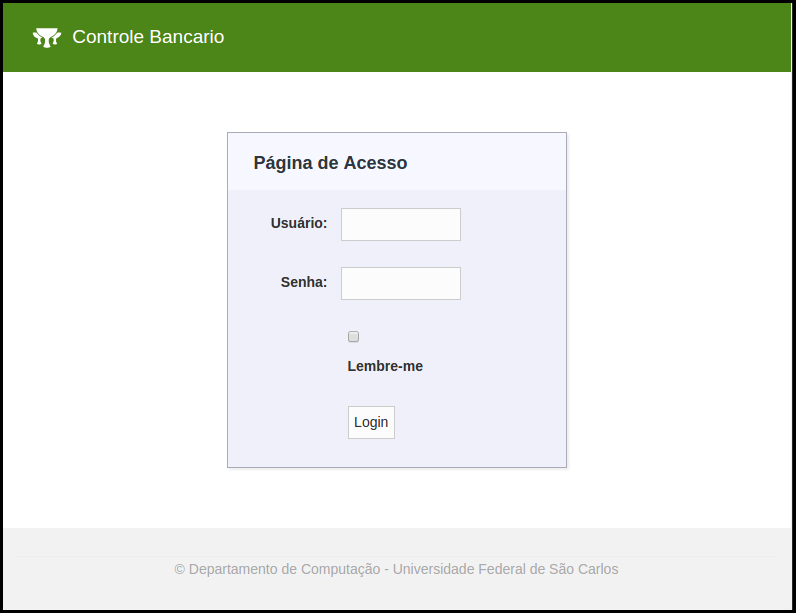
\includegraphics[width=14cm]{Login}
\caption{{\bf ControleBancario}: Página de {\it Login}}
\label{figExecutar}
\end{figure}

\section{Considerações finais}

\vspace{0.3cm}

Esse capítulo  apresentou a  segunda versão da  implementação da  aplicação {\bf
  ControleBancario}.         O        código-fonte        dessa        aplicação
({\footnotesize\texttt{ControleBancarioV2.zip}}) encontra-se  disponível no {\it
  Moodle}         do        curso,        localizado         no        endereço:
{\footnotesize\url{http://moodle.latosensu.dc.ufscar.br}}. Seguindo os passos do
tutorial   apresentado   obtem-se   esse   mesmo  código   da   aplicação   {\bf
  ControleBancario}.  

Dando continuidade ao desenvolvimento em  Grails, o próximo capítulo apresenta a
implementação   de  novas   funcionalidades  no   contexto  da   aplicação  {\bf
  ControleBancario}. 
